\documentclass{beamer}
\usepackage[utf8]{inputenc}
\usepackage{graphicx}
\begin{document}
%-----------------------------------------------------------------------------------------------------


\section*{Front End}
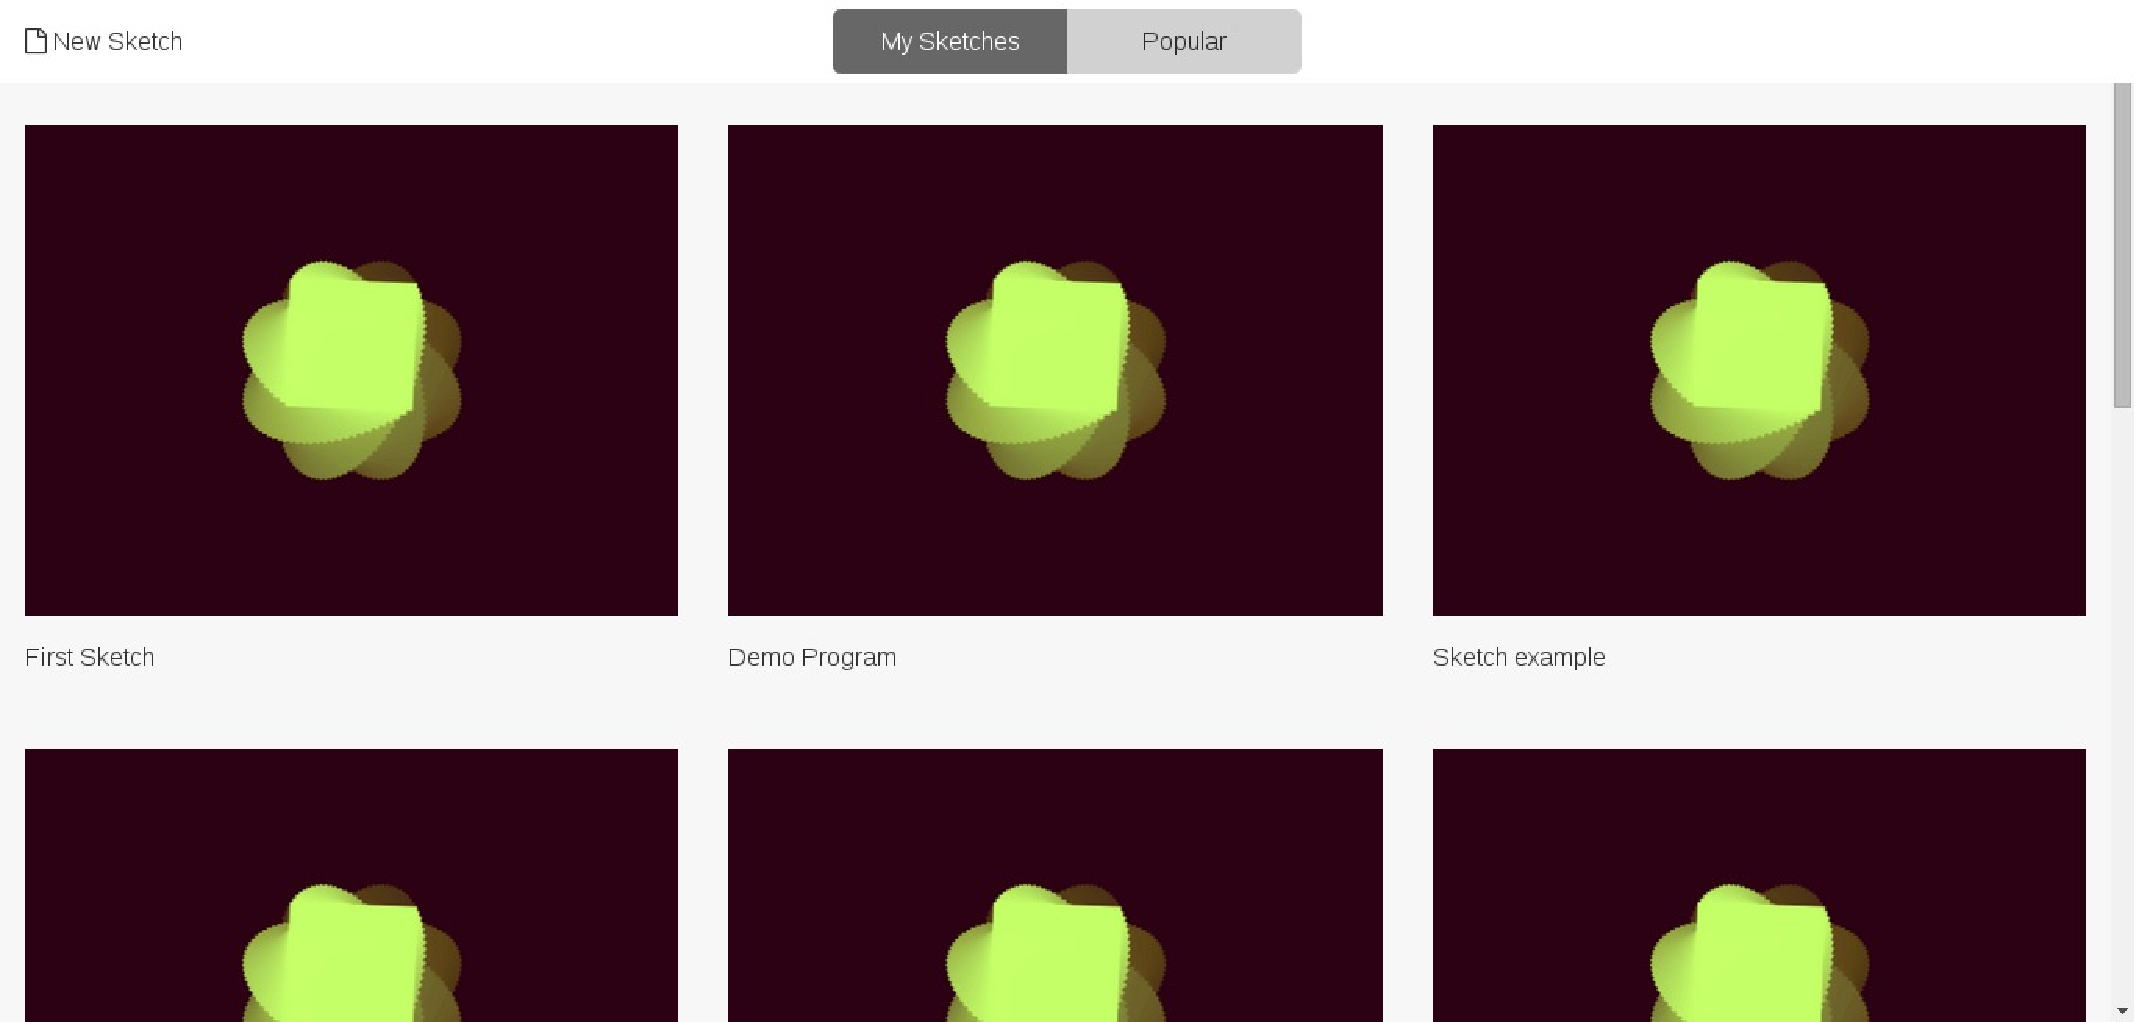
\includegraphics[width=\textwidth,keepaspectratio]{browser.pdf}
\hfill\\
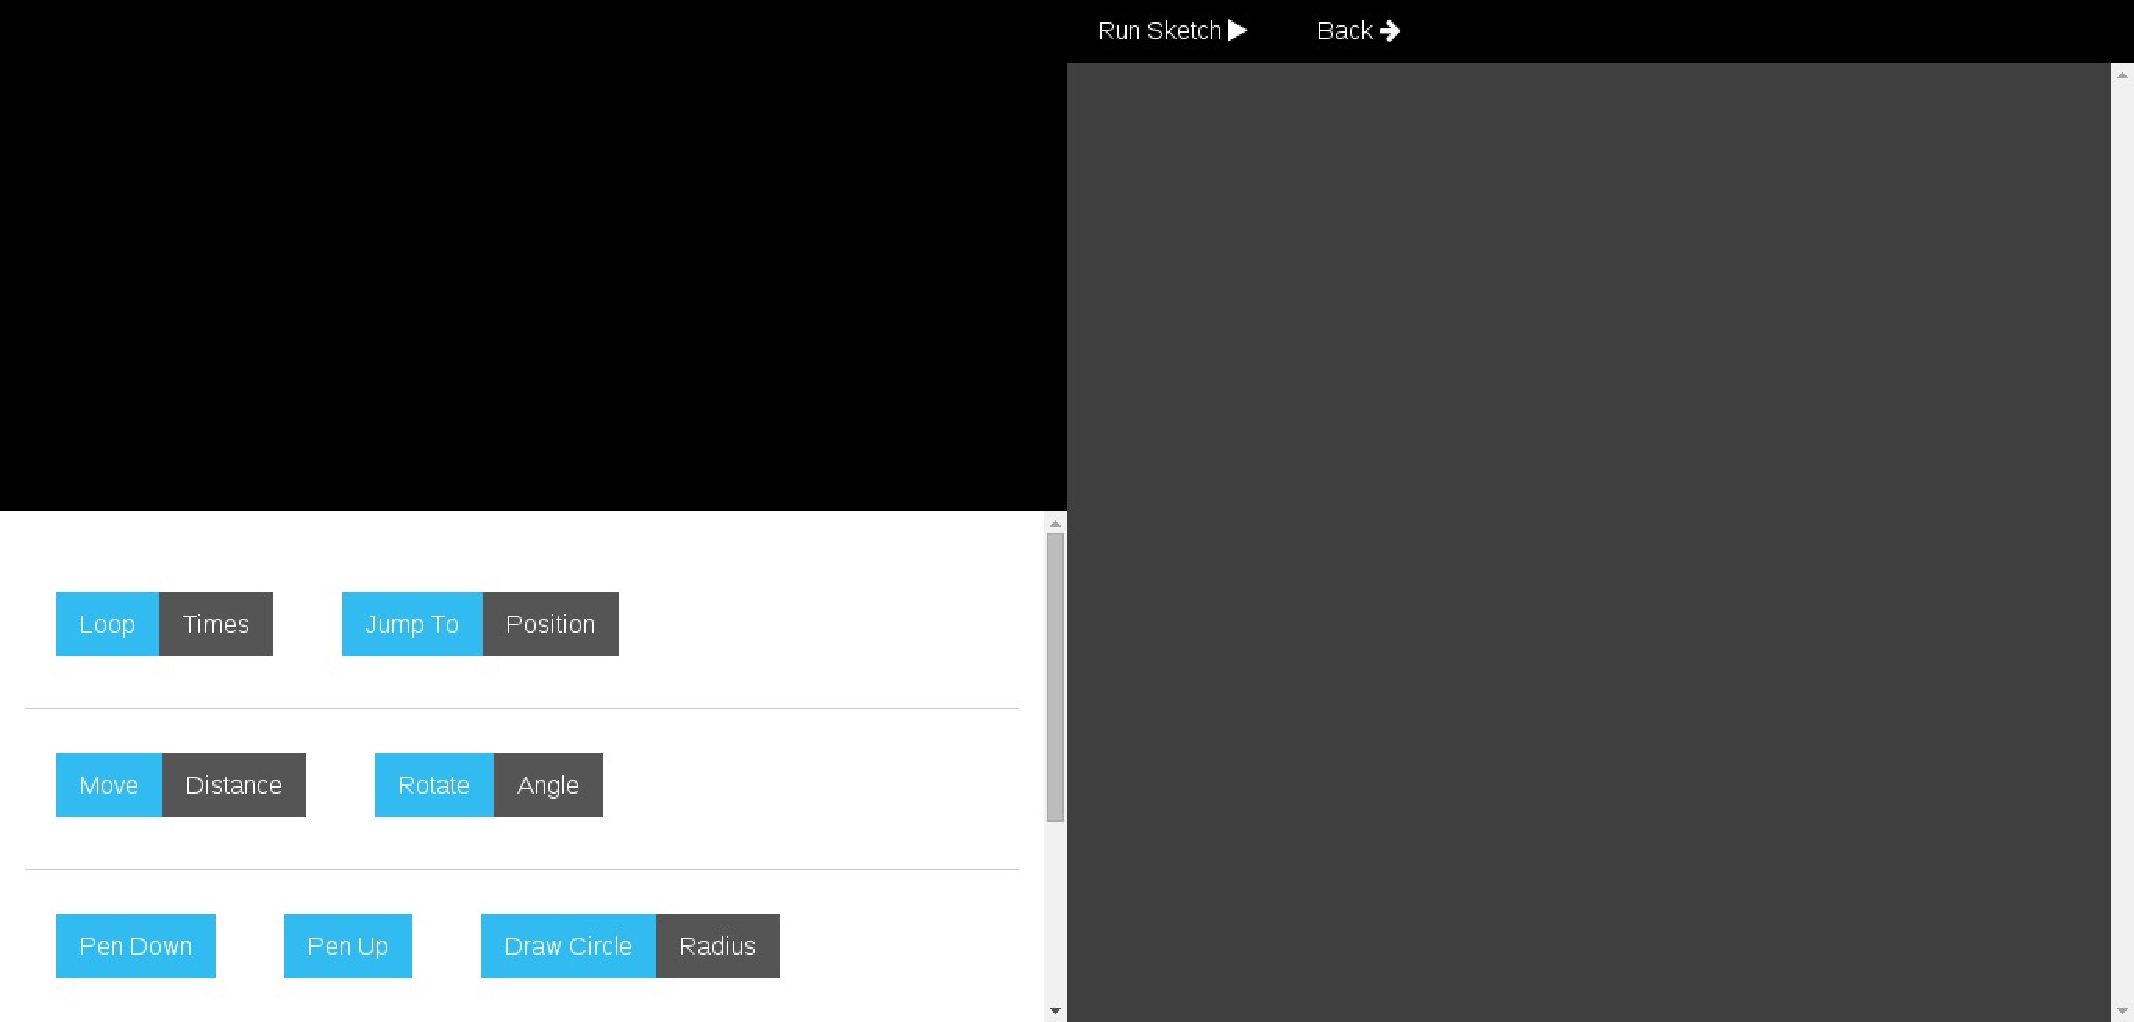
\includegraphics[width=\textwidth,keepaspectratio]{editor.pdf}
\hfill\\
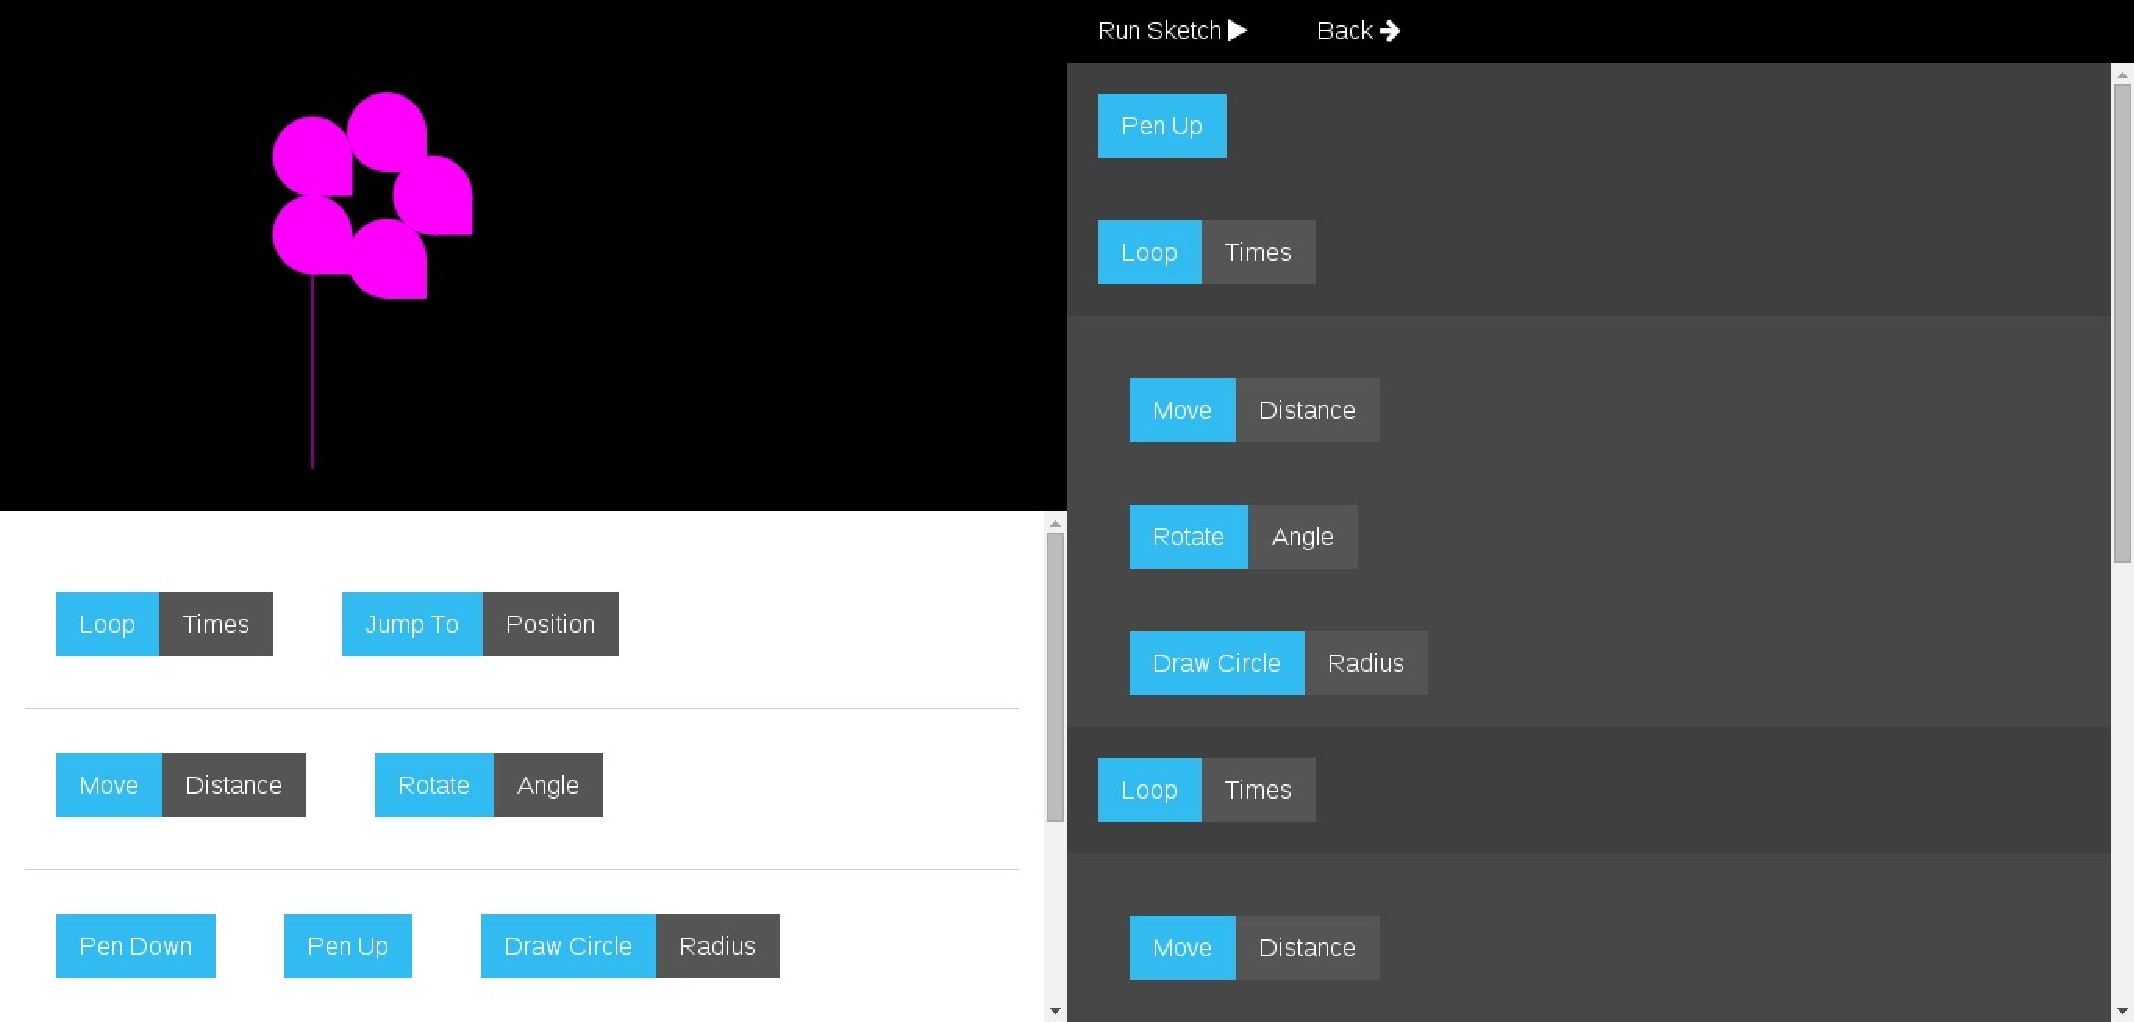
\includegraphics[width=\textwidth,keepaspectratio]{editor_with_contents.pdf}

\newpage
\section*{System Architecture.}
  \begin{itemize}
    \item Hosted on Heroku.
    \item Logical tier is NodeJS.
    \item Data tier is PostgreSQL.
    \item Preview images stored on Amazon S3
  \end{itemize}


\newpage
\section*{Scalability.}
  \begin{itemize}
    \item Stateless protocol.
    \item Client side computation.
    \begin{itemize}
      \item Images are encoded on the client side.
    \end{itemize}
    \item Caching.
    \begin{itemize}
	\item User sketches are stored locally.
    \end{itemize}
   \end{itemize}

\newpage
\section*{Security.}
  \begin{itemize}
    \item SQL text Input presented to PostgreSQL is parametrized to sanitize and avoid SQL injection.
    \item Escaping on the client side to avoid XSS.
  \end{itemize}
We have identified the need to provide authentication of devices to prevent unauthorized access to  user data.

\subsubsection*{Potential vulnerabilitys}
\begin{itemize}
  \item Issues with binary blob for preview images
  \item
\end{itemize}

\newpage
\section*{Reliability.}
  \begin{itemize}
    \item Running on Heroku.
    \item Testing
    \item Strategies for dealing with DOS
      \begin{itemize}
        \item Rate limiting?
        \item Data constraints?
      \end{itemize}
\end{itemize}

\newpage
\section*{Privacy.}
We have opted to store no personal information, except for a UUID which is tied to the device.


\newpage
\section*{Testing.}
 Demos!

%-----------------------------------------------------------------------------------------------------
\end{document}
